\chapter{Arhitektura i dizajn sustava}
	
	Za ostvarenje naše aplikacije odabrali smo arhitekturu zasnovanu na događajima. Prednosti ovog tipa arhitekture su mnoge: 
	\begin{itemize}
		\item svaki od servisa arhitekture može biti neovisan entitet, što povećava fleksibilnost 
		\item događaji se mogu pratiti u stvarnom vremenu, što olakšava analizu sustava
		\item događaji predstavljaju promjene stanja pa je komponentama omogućeno da reagiraju na te promjene
	\end{itemize}
	
				\begin{figure}[H]
			\includegraphics[scale=0.4]{slike/event\_driven\_architecture.PNG} %veličina slike u odnosu na originalnu datoteku i pozicija slike
			\centering
			\caption{Prikaz arhitekture zasnovane na događajima}
			\label{event_driven_architecture}
		\end{figure}
		
	Specifično, radi se o MVC (Model-View-Controller) obrascu, koji odvaja korisničko sučelje od ostatka sustava. On dodatno smanjuje međuovisnost U/I sučelja i ostatka sustava. Sastoji se od tri dijela:
	
		\begin{itemize}
			\item model - sadrži razrede čiji se objekti obrađuju
			\item view (pogled) - sadrži razrede čiji objekti služe za prikaz podataka (korisničko sučelje)
			\item controller (nadglednik) - sadrži razrede koji upravljaju i rukuju korisničkom interakcijom s pogledom i modelom
		\end{itemize}
		
			\begin{figure}[H]
			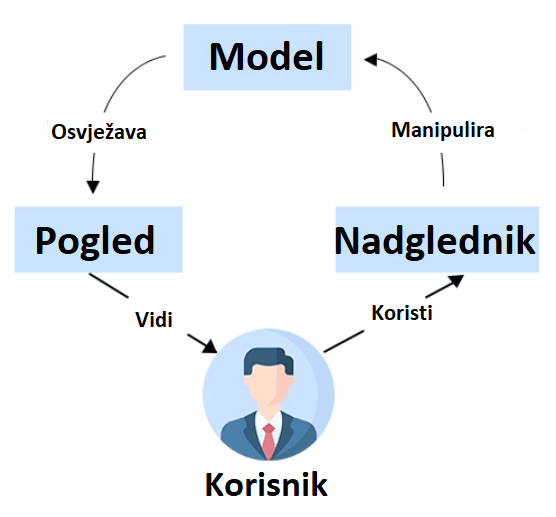
\includegraphics[scale=0.4]{slike/mvc.PNG} %veličina slike u odnosu na originalnu datoteku i pozicija slike
			\centering
			\caption{Prikaz načina rada MVC obrasca}
			\label{mvc}
		\end{figure}
		
	Po principu oblikovanja arhitekture odabrali smo \textit{Podijeli pa vladaj} arhitekturu, kako bismo se unutar tima mogli podijeliti u manje timove koji rade na određenim problemima i kako bismo, ako to bude bilo potrebno, jednostavno zamijenili željene dijelove bez opsežne intervencije u cijeli sustav.
	
			\begin{figure}[H]
			\includegraphics[scale=0.4]{slike/divide\_and\_conquer.PNG} %veličina slike u odnosu na originalnu datoteku i pozicija slike
			\centering
			\caption{Prikaz principa djelovanja "podijeli pa vladaj"}
			\label{divide_and_conquer}
		\end{figure}
		
	Arhitektura našeg sustava dijeli se na tri komponente:
	\begin{itemize}
		\item Web preglednik - softverska aplikacija koja omogućuje korisnicima pregledavanje i interakciju sa svim sadržajima Interneta. Glavna funkcija web preglednika je prikazivanje web stranica koje su oblikovane u obliku programskog koda na korisniku jasan način. Neki poznati web-preglednici uključuju Google Chrome, Mozilla Firefox, Opera...Web preglednik služi i kao medijator između korisnika, koji šalje zahtjeve, i web poslužitelja, koji prima zahtjeve i na njih odgovara.
		\item Web poslužitelj - program koji prosljeđuje web sadržaje web klijentu/pregledniku na njegov zahtjev putem protokola HTTP. On od klijenta dobije zahtjev za podacima, pristupa bazi podataka (kojoj također ima pristup), dohvaća tražene podatke iz baze te ih vraća klijentu u obliku HTTP odgovora. Vraćeni podaci se zatim prikazuju klijentu (ako nije došlo do poteškoća).
		\item Baza podataka - omogućuje organiziranu pohranu podataka koje je potrebno pohraniti (za KuhajIT su to podaci o korisničkim profilima, recepti, kuharice, osvrti na recepte, proizvodi i ostali)
	\end{itemize}
	
		\begin{figure}[H]
			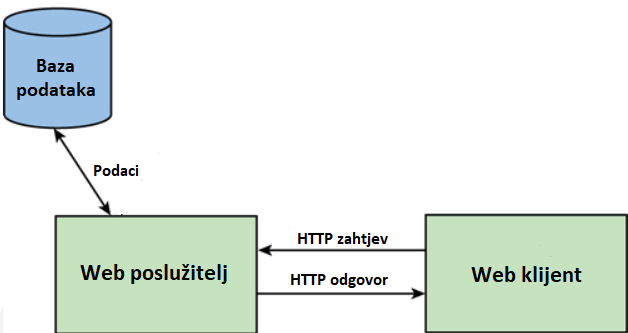
\includegraphics[scale=0.4]{slike/architecture.PNG} %veličina slike u odnosu na originalnu datoteku i pozicija slike
			\centering
			\caption{Prikaz principa djelovanja podsustava arhitekture}
			\label{architecture}
		\end{figure}
	
	
	
	Čitavi backend naše aplikacije izrađen je u programskom jeziku Java, u radnom okviru Spring. Razvojno okruženje korišteno za backend je Eclipse IDE.
	Frontend je izrađen u JavaScriptu, u biblioteci React. Razvojno okruženje korišteno za frontend je Visual Studio Code.
			
		\section{Baza podataka}

		Za ostvarenje naše aplikacije KuhajIT odabrali smo relacijsku bazu podataka PostgreSQL, koja svojom jednostavnom i lako razumljivom strukturom olakšava pregled i upravljanje podacima. Ključne komponente relacijske baze podataka su entiteti (tablice okarakterizirane imenom i skupom atributa) te veze među entitetima (strukture koje povezuju podatke iz različitih entiteta pomoću ključeva).
		
		Entiteti naše baze podataka su:
		\begin{itemize}
			\item User
			\item Recipe
			\item Recipe Ingredient
			\item Ingredient
			\item Cookbook
			\item Cookbook Recipe
			\item Review
			\item Response
			\item Image
		\end{itemize}
		
		
			\subsection{Opis tablica}
				
				\textbf{User} Entitet \textit{User} sadrži atribute važne za svakog registriranog korisnika aplikacije KuhajIT. Ti atributi su: ID korisnika, korisničko ime, lozinku, ime, prezime, email, uloga, biografija, url osobne fotografije i oznaka potvrđenosti. U vezi je \textit{One-to-Many} s entitetom \textit{Review} preko korisničkog ID-ja, \textit{One-to-Many} s entitetom \textit{Cookbook} preko korisničkog ID-ja, \textit{Recipe} preko korisničkog ID-ja i \textit{One-to-Many} s entitetom \textit{Response} preko korisničkog ID-ja.
				
				\begin{longtblr}[
					label=none,
					entry=none
					]{
						width = \textwidth,
						colspec={|X[6,l]|X[6, l]|X[20, l]|}, 
						rowhead = 1,
					} %definicija širine tablice, širine stupaca, poravnanje i broja redaka naslova tablice
					\hline \SetCell[c=3]{c}{\textbf{User}}	 \\ \hline[3pt]
					\SetCell{LightGreen}id & INT	&  	ID korisnika, sekvencijski generiran.  	\\ \hline
					username 	& VARCHAR &  Korisničko ime korisnika, koje mora biti jedinstveno, korisnik si ga bira sam pri registraciji, no može ga promijeniti. 	\\ \hline 
					password & VARCHAR & Lozinka za pristup korisničkom računu. \\
\hline
					name & VARCHAR	&  	Ime korisnika	\\ \hline 
					surname & VARCHAR & Prezime korisnika \\
\hline
					role & VARCHAR & Uloga koju neregistrirani korisnik želi imati (nutricionist, kulinarski entuzijast ili klijent). \\
\hline

					email & VARCHAR &   Ako se korisnik želi registrirati kao kulinarski entuzijast/nutricionist, mora priložiti email, inače atribut poprima NULL vrijednost.\\ \hline 
					slika & VARCHAR & Ako se korisnik želi registrirati kao kulinarski entuzijast/nutricionist, mora priložiti osobnu fotografiju, čiji se URL sprema u bazu, inače atribut poprima NULL vrijednost.\\
\hline

					biografija & VARCHAR & Ako se korisnik želi registrirati kao kulinarski entuzijast/nutricionist, mora priložiti kratku biografiju, inače atribut poprima NULL vrijednost.\\
\hline
				\end{longtblr}
				
				\textbf{Recipe} Entitet \textit{Recipe} sadrži atribute važne za svaki recept objavljen na web aplikaciji KuhajIT. Ti atributi su: ID recepta, ime recepta, vrijeme pripreme, koraci pripreme, ID autora recepta i veličina porcije. U vezi je \textit{One-to-Many} s entitetom \textit{Image} preko ID-ja recepta, \textit{One-to-Many} s entitetom \textit{Cookbook Recipe} preko ID-ja recepta, \textit{One-to-Many} s entitetom \textit{Recipe Ingredient} preko ID-ja recepta i \textit{Many-to-One} s entitetom \textit{User} preko ID-ja korisnika.
				
					\begin{longtblr}[
					label=none,
					entry=none
					]{
						width = \textwidth,
						colspec={|X[8,l]|X[6, l]|X[20, l]|}, 
						rowhead = 1,
					} %definicija širine tablice, širine stupaca, poravnanje i broja redaka naslova tablice
					\hline \SetCell[c=3]{c}{\textbf{Recipe}}	 \\ \hline[3pt]
					\SetCell{LightGreen}id & INT	&  Jedinstveni	ID recepta, sekvencijski generiran.  	\\ 
\hline
					cook\_time 	& INT &  Vrijeme pripreme recepta. 	\\ 
\hline 
					portion\_size & INT & Veličina porcije pripremljenog recepta. \\
\hline
					steps\_of\_making & VARCHAR	&  Koraci pripreme recepta.	\\ 
\hline 
					\SetCell{LightBlue}creator\_id	& INT &   Korisnički ID autora recepta.	\\ 
\hline 
				\end{longtblr}
				
				\textbf{Recipe Ingredient} Entitet \textit{Recipe Ingredient} sadrži atribute važne za pohranu sastojaka koji se koriste u pojedinom receptu objavljenom na web aplikaciji KuhajIT. Ti atributi su: ID sastojka recepta, količina sastojka, ID recepta i ID sastojka. U vezi je \textit{Many-to-One} s entitetom \textit{Recipe} preko ID-ja recepta i \textit{Many-to-One} s entitetom \textit{Ingredient}.
				
				\begin{longtblr}[
					label=none,
					entry=none
					]{
						width = \textwidth,
						colspec={|X[6,l]|X[6, l]|X[20, l]|}, 
						rowhead = 1,
					} %definicija širine tablice, širine stupaca, poravnanje i broja redaka naslova tablice
					\hline \SetCell[c=3]{c}{\textbf{Recipe Ingredient}}	 \\ \hline[3pt]
					\SetCell{LightGreen}id & INT	&  Jedinstveni ID sastojka recepta, sekvencijski generiran.  	\\ \hline
					quantity & INT &  Količina sastojka potrebnog za recept. 	\\ \hline 
					\SetCell{LightBlue}ingredient\_id	& INT &   ID sastojka.	\\ \hline
					\SetCell{LightBlue}recipe\_id	& INT & ID recepta. \\ \hline
				\end{longtblr}
				
				\textbf{Ingredient} Entitet \textit{Ingredient} sadrži atribute važne za svaki sastojak.
Ti atributi su: ID sastojka i ime sastojka. U vezi je \textit{One-to-Many} s entitetom \textit{Recipe Ingredient} preko ID-ja sastojka.

				\begin{longtblr}[
					label=none,
					entry=none
					]{
						width = \textwidth,
						colspec={|X[6,l]|X[6, l]|X[20, l]|}, 
						rowhead = 1,
					} %definicija širine tablice, širine stupaca, poravnanje i broja redaka naslova tablice
					\hline \SetCell[c=3]{c}{\textbf{Ingredient}}	 \\ \hline[3pt]
					\SetCell{LightGreen}id & INT	&  Jedinstveni ID sastojka, sekvencijski generiran.  	\\ \hline
					name 	& VARCHAR &  Naziv sastojka. 	\\ \hline 
				\end{longtblr}	
				
				\textbf{Cookbook} Entitet \textit{Cookbook} sadrži atribute važne za svaku kuharicu stvorenu od kulinarskog entuzijasta na web aplikaciji KuhajIT.
Ti atributi su: id kuharice, kategorija kuharice, naziv kuharice i id autora. U vezi je \textit{One-to-Many} s entitetom \textit{Cookbook Recipe} preko ID-ja kuharice i \textit{Many-to-One} s entitetom \textit{User} preko ID-ja korisnika (kulinarskog entuzijasta koji ju je stvorio).

				\begin{longtblr}[
					label=none,
					entry=none
					]{
						width = \textwidth,
						colspec={|X[6,l]|X[6, l]|X[20, l]|}, 
						rowhead = 1,
					} %definicija širine tablice, širine stupaca, poravnanje i broja redaka naslova tablice
					\hline \SetCell[c=3]{c}{\textbf{Cookbook}}	 \\ \hline[3pt]
					\SetCell{LightGreen}id & INT	&  Jedinstveni ID kuharice, sekvencijski generiran.  	\\ \hline
					category 	& VARCHAR &  Kategorija kuharice. 	\\ \hline 
					
					name & VARCHAR & Naziv kuharice. \\ \hline
					\SetCell{LightBlue}creator\_id	& INT &   Korisnički ID autora kuharice.	\\ \hline 
					
				\end{longtblr}
				
		\textbf{Cookbook Recipe} Entitet \textit{Cookbook Recipe} sadrži atribute važne za pohranu recepata u pojedinu kuharicu na web aplikaciji KuhajIT.
Ti atributi su: ID kuharice i ID recepta. U vezi je \textit{Many-to-One} s entitetom \textit{Cookbook} preko ID-ja kuharice i \textit{Many-to-One} s entitetom \textit{Recipe} preko ID-ja recepta koji se u kuharici nalazi.

			\begin{longtblr}[
					label=none,
					entry=none
					]{
						width = \textwidth,
						colspec={|X[6,l]|X[6, l]|X[20, l]|}, 
						rowhead = 1,
					} %definicija širine tablice, širine stupaca, poravnanje i broja redaka naslova tablice
					\hline \SetCell[c=3]{c}{\textbf{Cookbook Recipe}}	 \\ \hline[3pt]
					\SetCell{LightGreen}cookbook\_id & INT	&  ID kuharice.  	\\ \hline
					\SetCell{LightGreen}recipe\_id 	& INT &  ID recepta. 	\\ \hline				
				\end{longtblr}
				
				\textbf{Review} Entitet \textit{Review} sadrži atribute važne za svaku recenziju ostavljenu na recept na web aplikaciji KuhajIT.
Ti atributi su: ID recenzije, ocjena recepta dodijeljena u recenziji, poruka ostavljena u recenziji, ID autora recenzije i ID recepta na koji je recenzija ostavljena. U vezi je \textit{One-to-Many} s entitetom \textit{Cookbook Recipe} preko ID-ja kuharice i \textit{Many-to-One} s entitetom \textit{User} preko ID-ja korisnika koji je ostavio recenziju, \textit{Many-to-One} s entitetom \textit{Recipe} preko ID-ja recepta na koji je recenzija ostavljena i \textit{One-to-Many} s entitetom \textit{Response} preko ID-ja recenzije.

\begin{longtblr}[
					label=none,
					entry=none
					]{
						width = \textwidth,
						colspec={|X[6,l]|X[6, l]|X[20, l]|}, 
						rowhead = 1,
					} %definicija širine tablice, širine stupaca, poravnanje i broja redaka naslova tablice
					\hline \SetCell[c=3]{c}{\textbf{Review}}	 \\ \hline[3pt]
					\SetCell{LightGreen}id & INT	&  Jedinstveni ID recenzije, sekvencijski generiran.  	\\ \hline
					mark 	& INT &  Ocjena ostavljena u recenziji. 	\\ \hline 
					
					message & VARCHAR & Poruka ostavljena u recenziji. \\ \hline
					\SetCell{LightBlue}creator\_id & INT &   Korisnički ID autora recenzije, ako je recenziju ostavio neregistrirani korisnik, poprima vrijednost NULL.	\\ \hline 
					\SetCell{LightBlue} recipe\_id & INT &   ID recepta na kojeg je recenzija ostavljena.	\\ \hline 
					
				\end{longtblr}


\textbf{Response} Entitet \textit{Response} sadrži atribute važne za svaki odgovor na recenziju ostavljenu na recept na web aplikaciji KuhajIT.
Ti atributi su: ID odgovora, poruka ostavljena u odgovoru, ID autora odgovora (kulinarski entuzijast na čiji je recept ostavljena recenzija) i ID recenzije na koju je odgovor ostavljen. U vezi je \textit{Many-to-One} s entitetom \textit{Review} preko ID-ja recenzije i \textit{Many-to-One} s entitetom \textit{User} preko ID-ja korisnika koji odgovara na recenziju.
				
			\begin{longtblr}[
					label=none,
					entry=none
					]{
						width = \textwidth,
						colspec={|X[6,l]|X[6, l]|X[20, l]|}, 
						rowhead = 1,
					} %definicija širine tablice, širine stupaca, poravnanje i broja redaka naslova tablice
					\hline \SetCell[c=3]{c}{\textbf{Response}}	 \\ \hline[3pt]
					\SetCell{LightGreen}id & INT	&  Jedinstveni ID odgovora na recenziju, sekvencijski generiran.  	\\ \hline
					message & VARCHAR & Poruka ostavljena u odgovoru na recenziju. \\ \hline
					\SetCell{LightBlue}creator\_id	& INT &   Korisnički ID autora odgovora na recenziju.	\\ \hline 
					\SetCell{LightBlue}review\_id & INT &   ID recenzije na koju autor recepta odgovara.	\\ \hline 
					
				\end{longtblr}
				
				\textbf{Image} Entitet \textit{Image} sadrži atribute važne za svaku fotografiju učitanu u sklopu recepta na web aplikaciji KuhajIT.
Ti atributi su: ID fotografije, URL fotografije i ID recepta uz kojeg je fotografija učitana. U vezi je \textit{Many-to-One} s entitetom \textit{Recipe} preko ID-ja recepta.

				\begin{longtblr}[
					label=none,
					entry=none
					]{
						width = \textwidth,
						colspec={|X[6,l]|X[6, l]|X[20, l]|}, 
						rowhead = 1,
					} %definicija širine tablice, širine stupaca, poravnanje i broja redaka naslova tablice
					\hline \SetCell[c=3]{c}{\textbf{Image}}	 \\ \hline[3pt]
					\SetCell{LightGreen}id & INT	&  Jedinstveni ID učitane fotografije, sekvencijski generiran.  	\\ \hline

					url & VARCHAR & URL učitane fotografije. \\ \hline	
					\SetCell{LightBlue}recipe\_id	& INT &   ID recepta uz koji je fotografija učitana.	\\ \hline 	
				\end{longtblr}
				
				\eject	
	
	  \section{Dijagram razreda}
	  
	  \begin{figure}[H]
			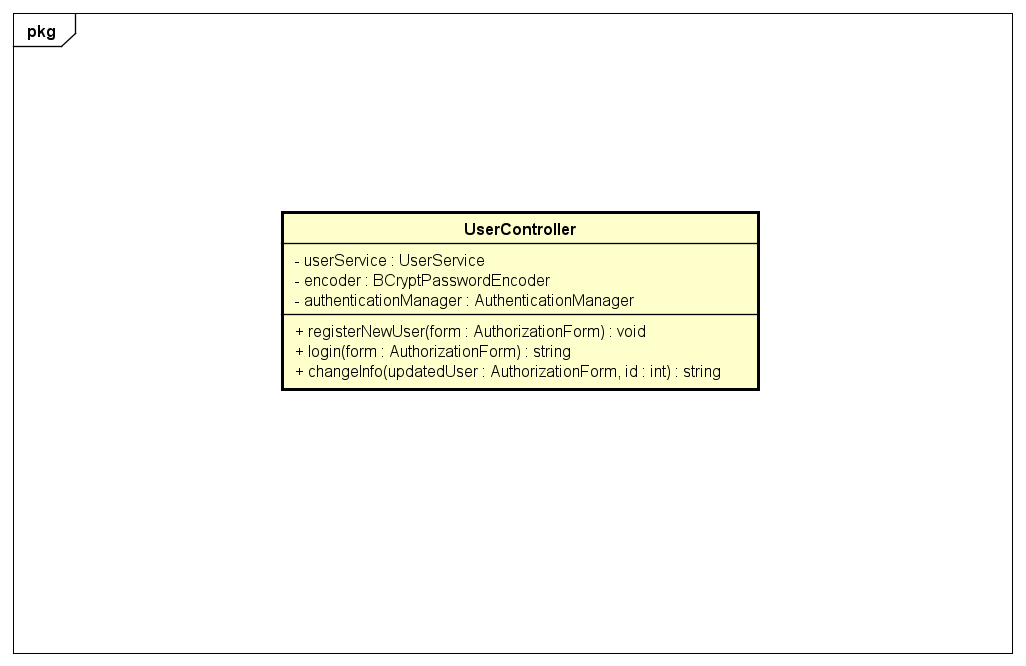
\includegraphics[scale=0.5]{dijagrami/UML_dijagram_razreda_controllers.png} %veličina slike u odnosu na originalnu datoteku i pozicija slike
			\centering
			\caption{Dijagram razreda - dio Controllers}
			\label{Dijagram razreda - dio Controllers}
		\end{figure}
			
			
			\eject 	
			
			
			\begin{figure}[H]
			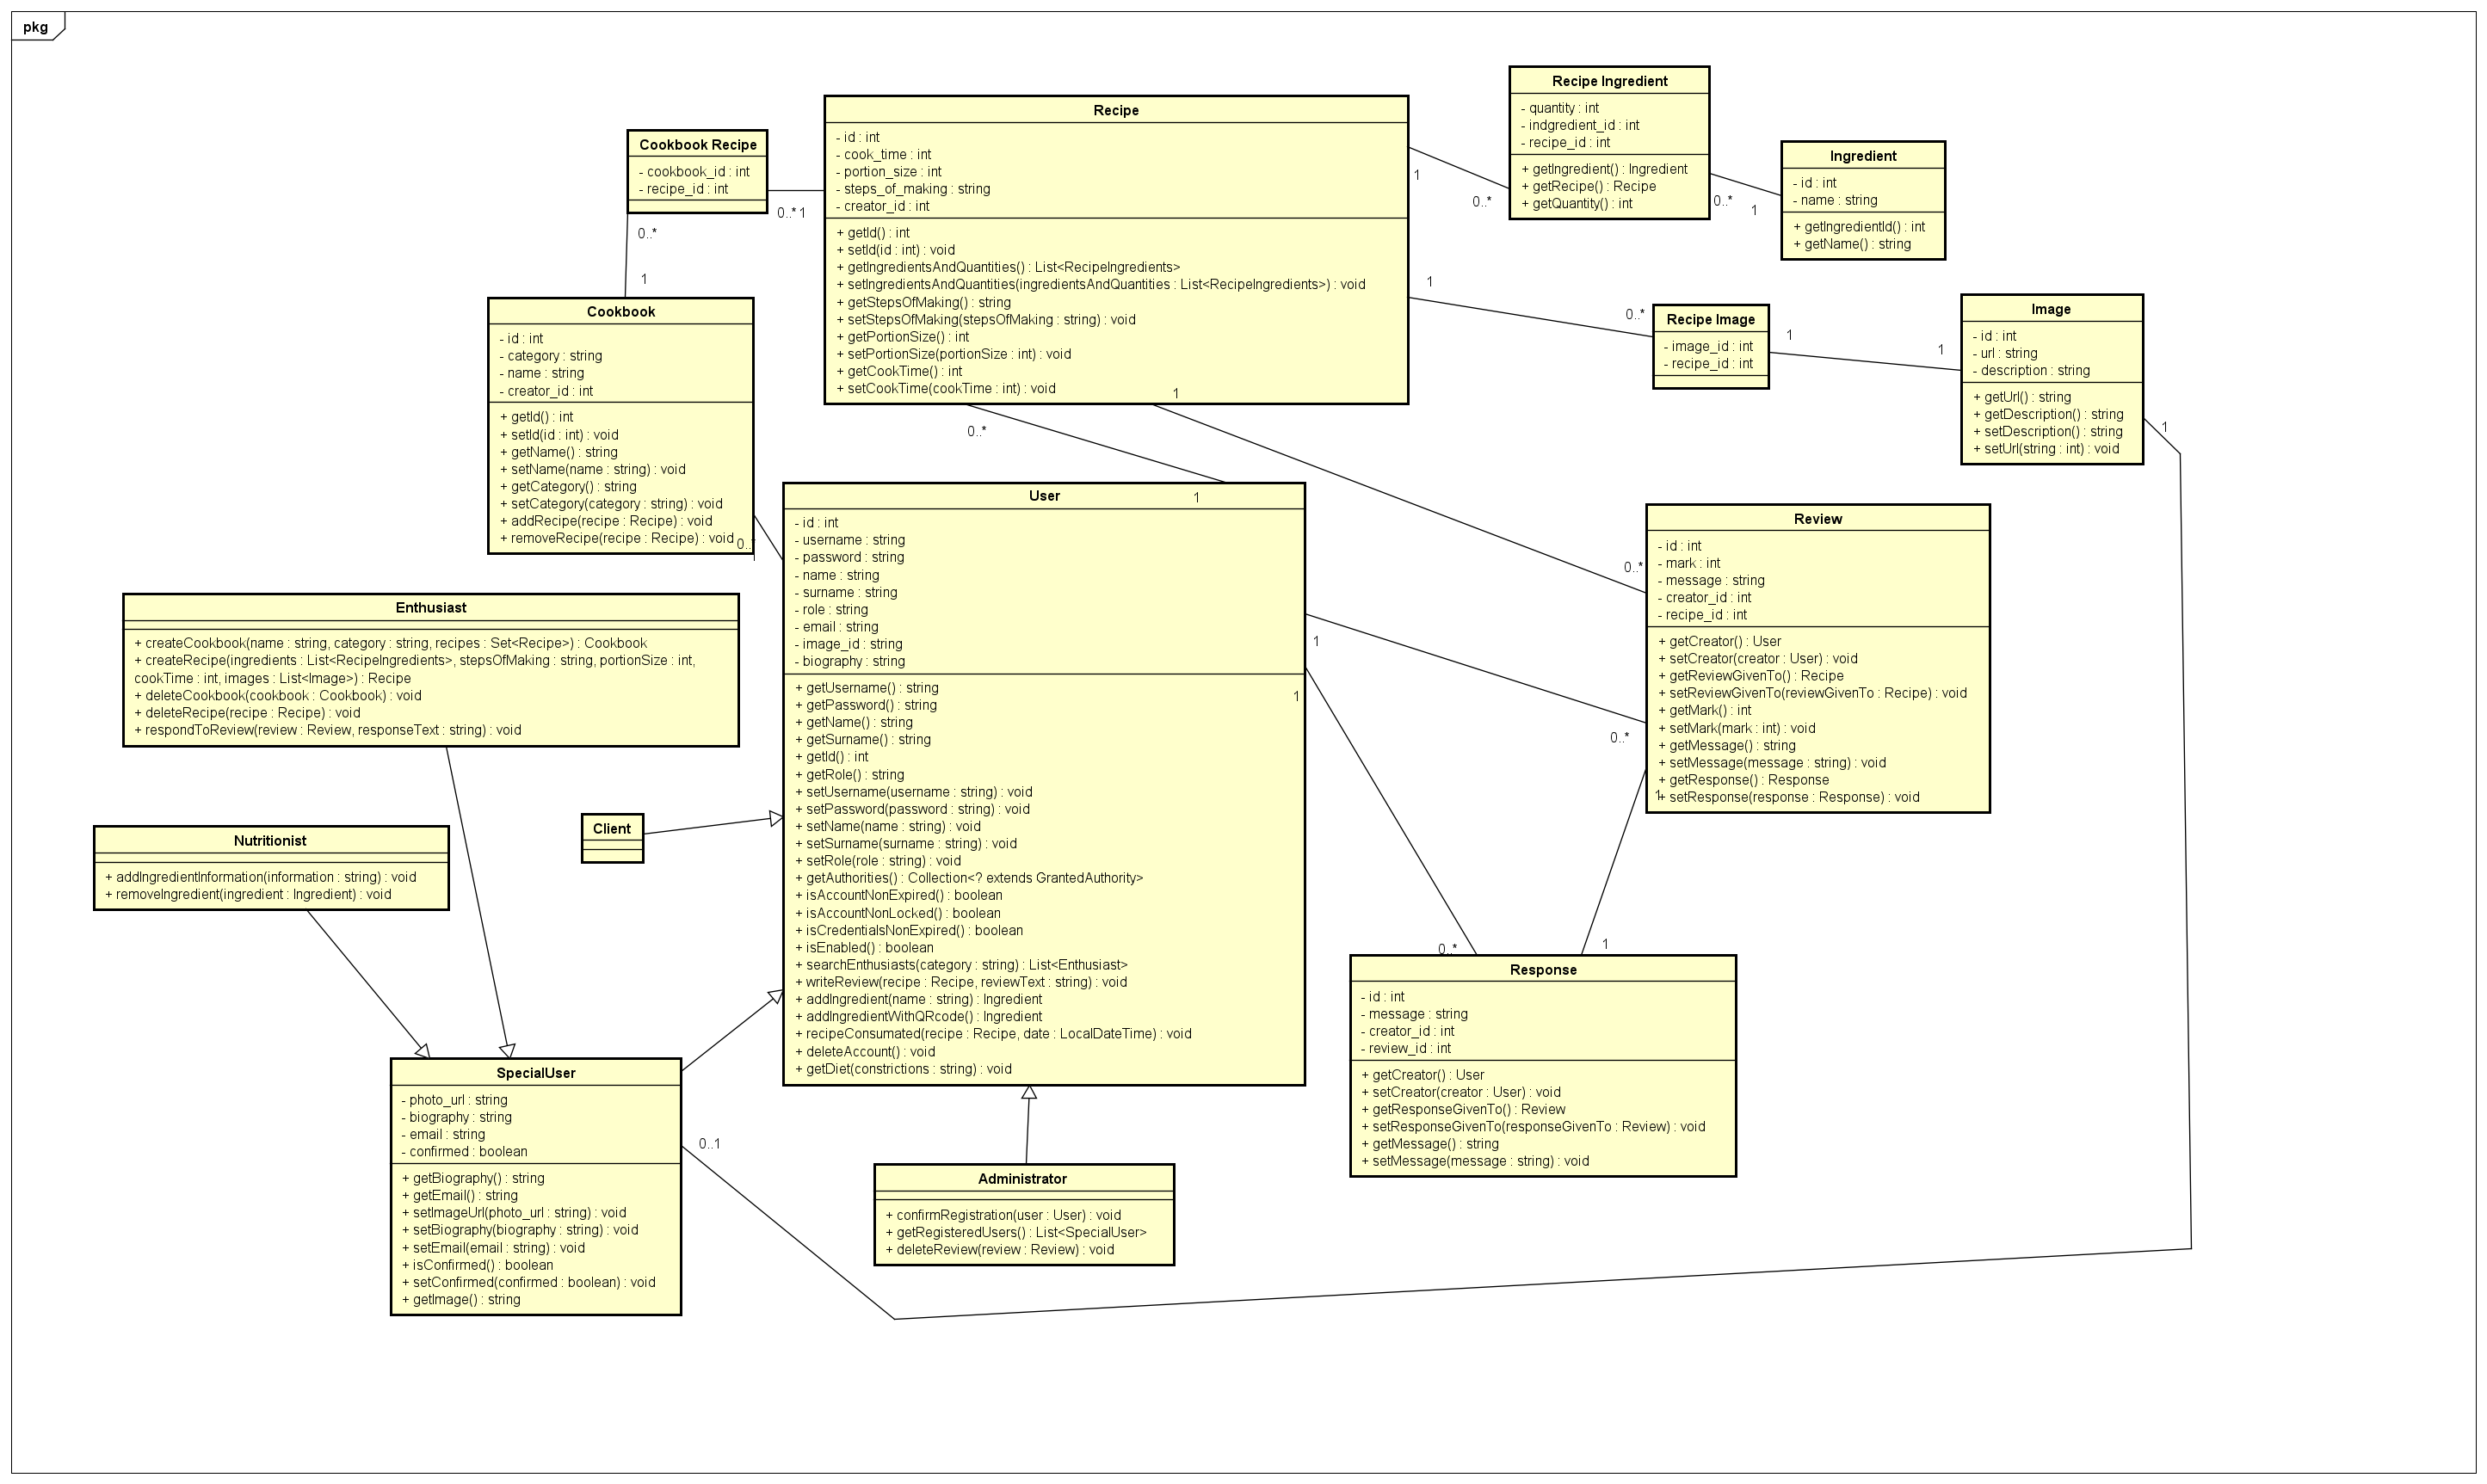
\includegraphics[scale=0.2]{dijagrami/UML_dijagram_razreda_models.png} %veličina slike u odnosu na originalnu datoteku i pozicija slike
			\centering
			\caption{Dijagram razreda - dio Models}
			\label{Dijagram razreda - dio Models}
		\end{figure}
			
			
			\eject 		
			
		\section{Dijagram stanja}
			
			
			\textbf{\textit{dio 2. revizije}}\\
			
			\textit{Potrebno je priložiti dijagram stanja i opisati ga. Dovoljan je jedan dijagram stanja koji prikazuje \textbf{značajan dio funkcionalnosti} sustava. Na primjer, stanja korisničkog sučelja i tijek korištenja neke ključne funkcionalnosti jesu značajan dio sustava, a registracija i prijava nisu. }
			
			
			\eject 
		
		\section{Dijagram aktivnosti}
			
			\textbf{\textit{dio 2. revizije}}\\
			
			 \textit{Potrebno je priložiti dijagram aktivnosti s pripadajućim opisom. Dijagram aktivnosti treba prikazivati značajan dio sustava.}
			
			\eject
		\section{Dijagram komponenti}
		
			\textbf{\textit{dio 2. revizije}}\\
		
			 \textit{Potrebno je priložiti dijagram komponenti s pripadajućim opisom. Dijagram komponenti treba prikazivati strukturu cijele aplikacije.}